\documentclass[tikz, border=3mm]{standalone}
\usetikzlibrary{positioning}

\usepackage{tikz-uml}

\begin{document}
  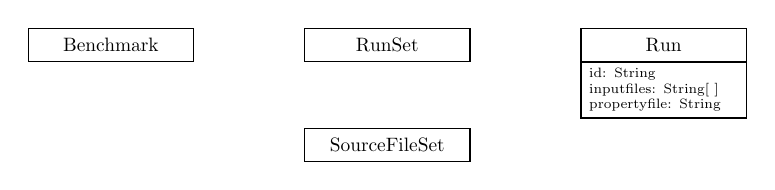
\begin{tikzpicture} [
        scale = 0.7,
        transform shape,
        node distance = 2cm,
        every node/.style = {
          align = center,
          %font = \footnotesize,
        },
        umlbox/.style = {
          draw,
          minimum width = 3cm,
          minimum height = 0.6cm,          
        }
      ]

    % textboxes
    \node [umlbox] (Benchmark) {Benchmark};
    \node [umlbox, right = of Benchmark] (RunSet) {RunSet};
    \node [umlbox, right = of RunSet] (Run) {Run};
    \node [umlbox, below = 0cm of Run, align=left, font=\scriptsize, text width = 2.7cm] (desc) {id: String\\inputfiles: String[\ ]\\propertyfile: String};
    \node [umlbox, below = 1.2cm of RunSet] (SourceFileSet) {SourceFileSet};

    % relations
    % for more configuration options regarding relations, c.f.
    % https://perso.ensta-paristech.fr/~kielbasi/tikzuml/var/files/html/web-tikz-uml-userguidech2.html
    \umlaggreg[geometry=--, arg2=1..n]{Benchmark}{RunSet};
    \umlaggreg[geometry=--]{RunSet}{SourceFileSet};
    \umlaggreg[geometry=--, arg2=1..n]{RunSet}{Run};
    \umlaggreg[geometry=-|-, anchor2=170, arg2=1..n, pos2=2.6]{SourceFileSet}{desc};

  \end{tikzpicture}
\end{document}
